\documentclass[a4paper, 11pt]{article}

\usepackage[margin=2cm]{geometry}
\usepackage{csquotes}
\usepackage[pdftex]{hyperref}

\UseRawInputEncoding
\usepackage{listings}
\usepackage{amssymb}
\usepackage[pdftex]{hyperref}
\usepackage[utf8]{inputenc}
\usepackage{ragged2e}
\usepackage{indentfirst}
\usepackage{listings}
\usepackage{xcolor}
\usepackage[brazilian]{babel}
\usepackage[style=abnt, backend=biber]{biblatex}
\addbibresource{ref.bib}
\usepackage{graphicx}
\usepackage{booktabs}
\usepackage{bm}
\usepackage{array}
\graphicspath{ {./images/} }
\usepackage{float}
\usepackage{amsmath}
\usepackage[pdftex]{hyperref}
\usepackage{longtable}
\DeclareMathOperator\arctanh{arctanh}
\usepackage{multicol}
\usepackage{caption}
\usepackage{subcaption}
\usepackage{wrapfig}

\usepackage{titlesec}

\setcounter{secnumdepth}{4} % Define a profundidade de numeração das seções
\titleclass{\subsubsubsection}{straight}[\subsection] % Define a classe para \subsubsubsection
\newcounter{subsubsubsection}[subsubsection] % Cria um novo contador para \subsubsubsection
\renewcommand\thesubsubsubsection{\thesubsubsection.\arabic{subsubsubsection}} % Define a formatação do número

\titleformat{\subsubsubsection}
  {\normalfont\normalsize\bfseries}{\thesubsubsubsection}{1em}{} % Formatação do título
\titlespacing*{\subsubsubsection}
  {0pt}{3.25ex plus 1ex minus .2ex}{1.5ex plus .2ex} % Espaçamento antes e depois do título
\makeatletter
\renewcommand\paragraph{\@startsection{paragraph}{5}{\z@}%
  {3.25ex \@plus1ex \@minus.2ex}%
  {-1em}%
  {\normalfont\normalsize\bfseries}}
\renewcommand\subparagraph{\@startsection{subparagraph}{6}{\parindent}%
  {3.25ex \@plus1ex \@minus .2ex}%
  {-1em}%
  {\normalfont\normalsize\bfseries}}
\def\toclevel@subsubsubsection{4} % Define o nível no índice
\def\l@subsubsubsection{\@dottedtocline{4}{7em}{4em}} % Define a aparência no índice
\makeatother

\usepackage[T1]{fontenc} 


\definecolor{codegreen}{rgb}{0,0.6,0}
\definecolor{codegray}{rgb}{0.5,0.5,0.5}
\definecolor{codepurple}{rgb}{0.58,0,0.82}
\definecolor{backcolour}{rgb}{0.95,0.95,0.92}

\definecolor{mGreen}{rgb}{0,0.6,0}
\definecolor{mGray}{rgb}{0.5,0.5,0.5}
\definecolor{mPurple}{rgb}{0.58,0,0.82}
\definecolor{backgroundColour}{rgb}{0.95,0.95,0.92}

\lstdefinestyle{CStyle}{
    backgroundcolor=\color{backgroundColour},   
    commentstyle=\color{mGreen},
    keywordstyle=\color{magenta},
    numberstyle=\tiny\color{mGray},
    stringstyle=\color{mPurple},
    basicstyle=\footnotesize,
    breakatwhitespace=false,         
    breaklines=true,                 
    captionpos=b,                    
    keepspaces=true,                 
    numbers=left,                    
    numbersep=5pt,                  
    showspaces=false,                
    showstringspaces=false,
    showtabs=false,                  
    tabsize=2,
    language=C
}

\lstset{style=CStyle
}
\def\therefore{\boldsymbol{\text{ }
\leavevmode
\lower0.4ex\hbox{$\cdot$}
\kern-.5em\raise0.7ex\hbox{$\cdot$}
\kern-0.55em\lower0.4ex\hbox{$\cdot$}
\thinspace\text{ }}}

\lstset{
    language=Matlab,
    literate=
    {á}{{\'a}}1 {é}{{\'e}}1 {í}{{\'i}}1 {ó}{{\'o}}1 {ú}{{\'u}}1
    {â}{{\^a}}1 {ê}{{\^e}}1 {ô}{{\^o}}1 {û}{{\^u}}1
    {ã}{{\~a}}1 {õ}{{\~o}}1
    {ç}{{\c c}}1 {Ç}{{\c C}}1
}

\begin{document}
    \begin{titlepage}
    	\begin{center}
            \begin{figure}[H]
                \centering
                
\includegraphics[width=7cm]{images/ufrj-logo.png}
                \hspace{1cm}
                
\includegraphics[width=5cm]{images/poli-logo.png}
            \end{figure}
            \vspace{85pt}
            
            
            \textbf{\LARGE{Acionamento de Máquina de Indução - Sensores II}}
            \large{\\}
            \vspace{50pt}
            \textbf{\LARGE{Grupo 4}}
            \large{\\}
            \vspace{160pt}
            
        \end{center}
        	
        \begin{flushleft}
        	\begin{tabbing}
        	    \\\\
        		Alunos\qquad\qquad\= \\
                \qquad\qquad Arthur Malta;  DRE:120046661\\
                \qquad\qquad Bruno Fraga; DRE: 120046653\\
                \qquad\qquad Gabriel José Souza e Silva; DRE: 118055329\\
                \qquad\qquad João Vitor Assumpção; DRE: 118062952\\
            \end{tabbing}
        \end{flushleft}
        	
        \begin{center}
        	\vspace{\fill}
        	    \today
        \end{center}
    \end{titlepage}
    %%%%%%%%%%%%%%%%%%%%%%%%%%%%%%%%%%%%%%%%%%%%%%%%%%%%%%%%%%%
    \newpage
    \tableofcontents
    \thispagestyle{empty}
    
    \newpage
    \pagenumbering{arabic}
    %%%%%%%%%%%%%%%%%%%%%%%%%%%%%%%%%%%%%%%%%%%%%%%%%%%%%%%%%
    %%%%%%%%%%%%%%%%%%%%%%%%%%%%%%%%%%%%%%%%%%%%%%%%%%%%
\section{Introdução}
  
Os \textit{soft starters} e os inversores de frequência (\textit{Variable Frequency Drives - VFDs}) são dispositivos utilizados para reduzir a corrente de partida de motores e controlar o torque, protegendo equipamentos conectados e prolongando a vida útil dos motores. No entanto, diferem significativamente em funcionalidades e aplicações. Os \textit{soft starters} controlam a tensão aplicada ao motor durante o início e término da operação, proporcionando um aumento gradual da velocidade e minimizando choques mecânicos. Eles são ideais para sistemas que necessitam de controle de torque apenas na partida e parada, como transportadores, sistemas de correias e tubulações, onde se busca evitar picos de torque e fenômenos como golpes de aríete. Por outro lado, os inversores de frequência oferecem controle total da velocidade do motor durante todo o ciclo operacional, ajustando a frequência e a tensão fornecidas. Isso os torna mais adequados para aplicações que exigem controle dinâmico de velocidade, como ventiladores, bombas e sistemas industriais. Além disso, os VFDs proporcionam significativas economias de energia em equipamentos centrífugos, devido à redução de potência proporcional ao cubo da velocidade do motor. Apesar de serem mais caros e ocuparem mais espaço, os VFDs oferecem benefícios adicionais, como funcionalidade \textit{PLC-like}, diagnósticos avançados e maior flexibilidade operacional. Assim, a escolha entre essas tecnologias depende das necessidades específicas da aplicação, do custo inicial e do ciclo de vida do sistema.
  
\section{Partida direta}

\subsection{Circuitos}

Para realizar a simulação do acionamento utilizando partida direta e inversor de frequência, foi empregado o modelo de uma máquina de indução trifásica, conforme apresentado na Figura \ref{máquina de indução}. 

\begin{figure}[H]
    \centering
        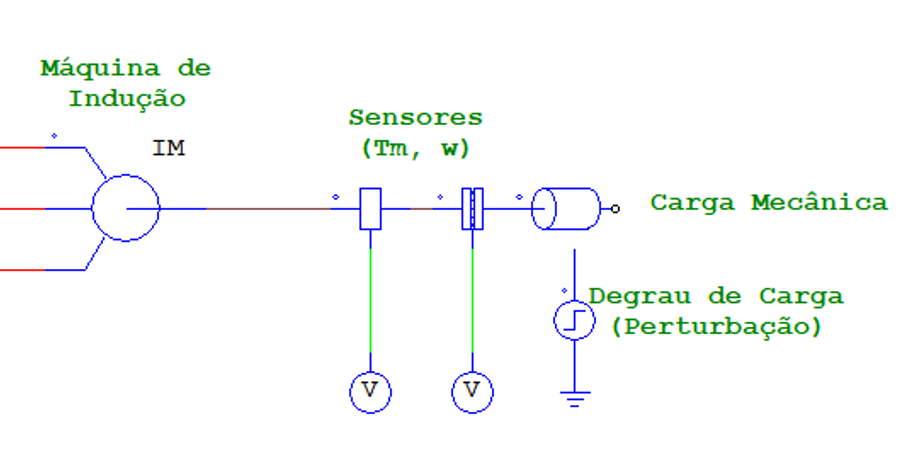
\includegraphics[width=1\linewidth]{images/máquina de indução (circuito).png}
    \caption{Máquina de indução.}
    \label{máquina de indução}
\end{figure}

Na partida direta, não há controle no processo de acionamento, e a máquina é conectada diretamente a uma fonte trifásica de alimentação. Nesse caso, o circuito é composto por uma máquina de indução ligada a três fontes de tensão senoidais, com defasagem de $120^\circ$ entre as fases e tensão de linha de 220 V RMS. O acionamento por partida direta pode ser visto na figura \ref{partida direta}

\begin{figure}[H]
    \centering
        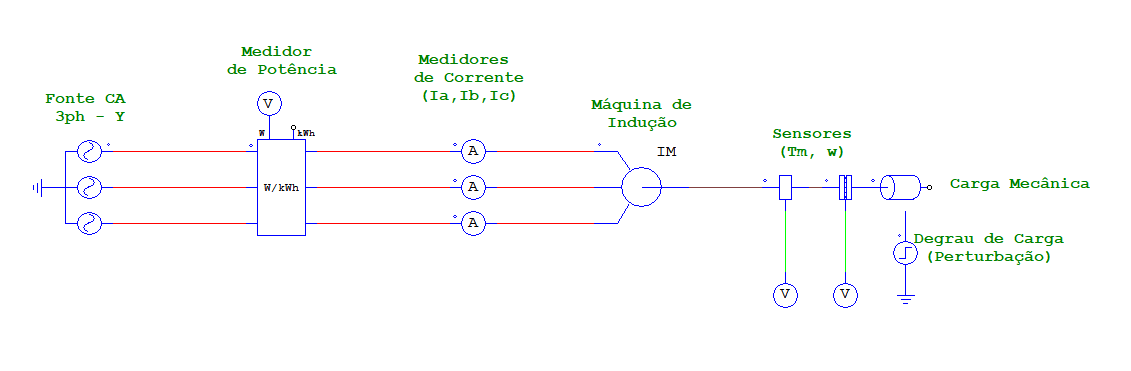
\includegraphics[width=1\linewidth]{images/partida direta circuito.png}
    \caption{Acionamento por partida direta.}
    \label{partida direta}
\end{figure}

A partida direta, apesar de ser uma solução simples para o acionamento de motores elétricos, possui uma limitação importante. A corrente durante a partida pode atingir valores várias vezes maior que a corrente nominal do motor. Os impactos desse comportamento podem ser observados tanto em outros dispositivos quanto em quedas de tensão na rede elétrica. Nas sessões seguintes veremos os resultados utilizados para contornar essas desvantagens e oferecer um acionamento mais controlado e moderado. 

\subsection{Resultados}

\subsubsection{Correntes trifásicas na partida direta.}

Nota-se pela figura \ref{correntes diretas} o elevado pico de corrente durante o transiente do acionamento.

\begin{figure}[H]
    \centering
    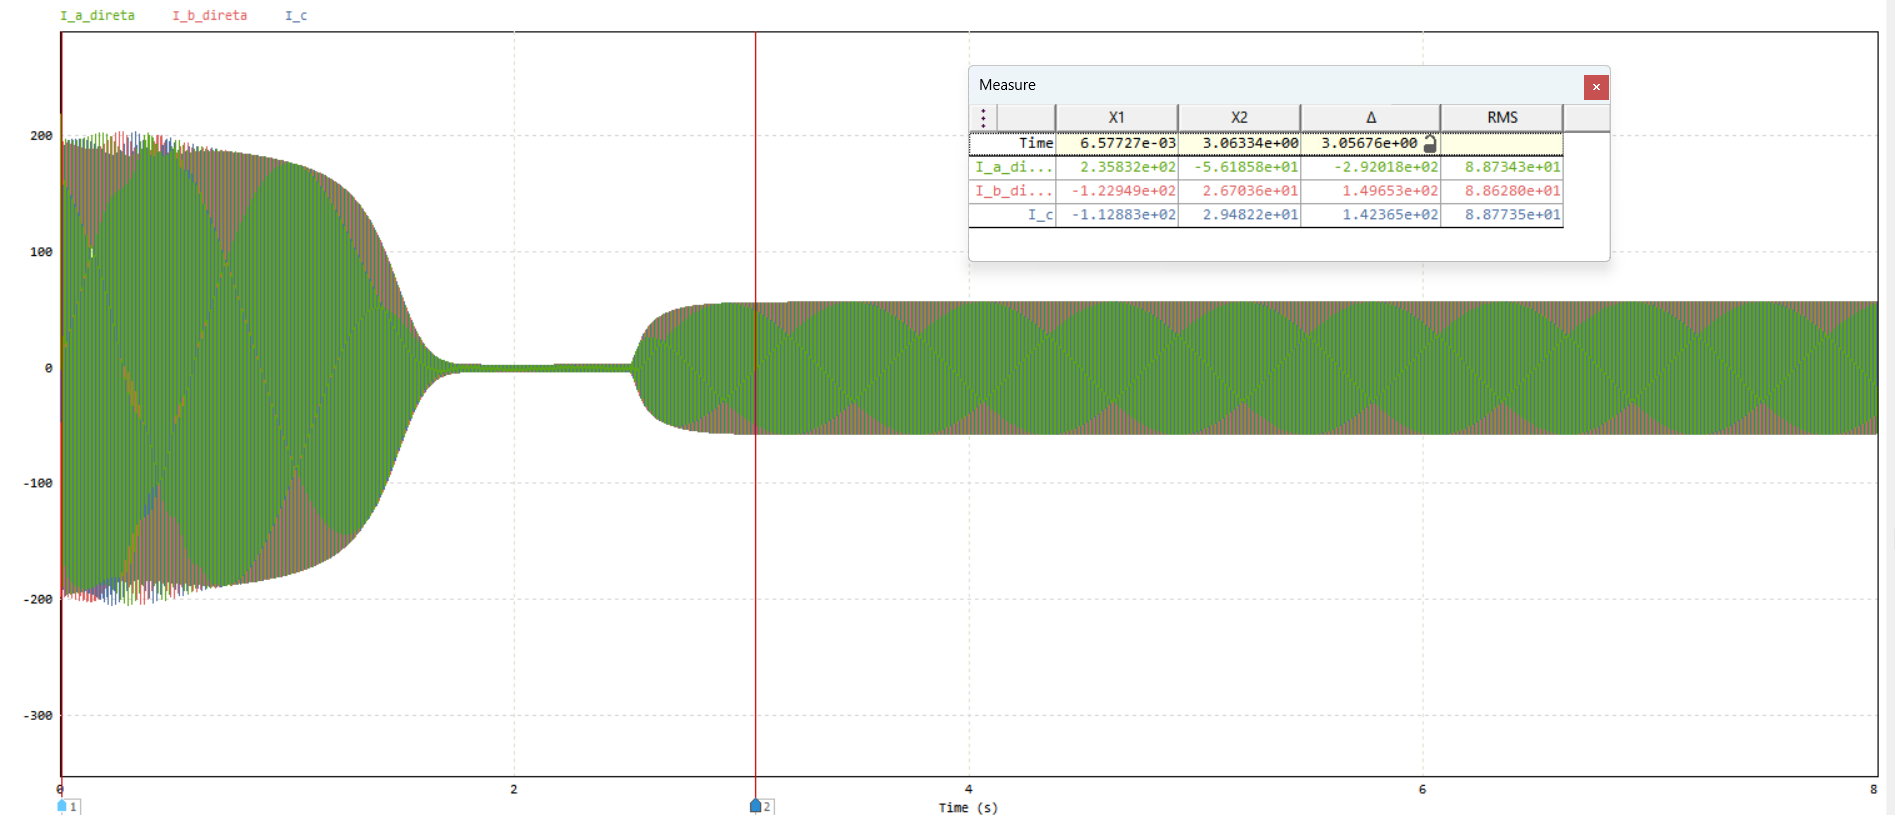
\includegraphics[width=1\linewidth]{images/correntes_diretas_novo.png}
    \caption{Correntes Ia, Ib e Ic [A] na partida direta.}
    \label{correntes diretas}
\end{figure}

Após o regime transiente, o motor, que parte a vazio, atinge uma velocidade constante de 1800 RPM (velocidade síncrona para um motor de 4 polos ligado na rede elétrica, cuja frequência é de 60 Hz). Nesse estado, as correntes trifásicas tendem a se aproximar de zero devido à ausência de carga. Entretanto, assim como feito para o acionamento por inversor de frequência, uma carga de 59 N·m foi aplicada ao sistema no instante de 2,5 segundos (o cálculo desse parâmetro será detalhado em seções posteriores). Consequentemente, observa-se um aumento nas correntes, refletindo a resposta do motor à carga aplicada.

\subsubsection{Velocidade do motor na partida direta.}
É possível observar que, partindo da inércia sem aplicação de carga, a velocidade assíncrona aumenta, sendo consumida em parte pelo escorregamento, maior no momento de inércia do motor. Uma vez atingida a velocidade objetivada, esta entra em regime permanente e o escorregamento torna-se nulo por não haver carga. A aplicação da carga no instante de 2.5 segundos, resulta na diminuição da velocidade em razão de um maior escorregamento.  

\begin{figure}[h]
    \centering
    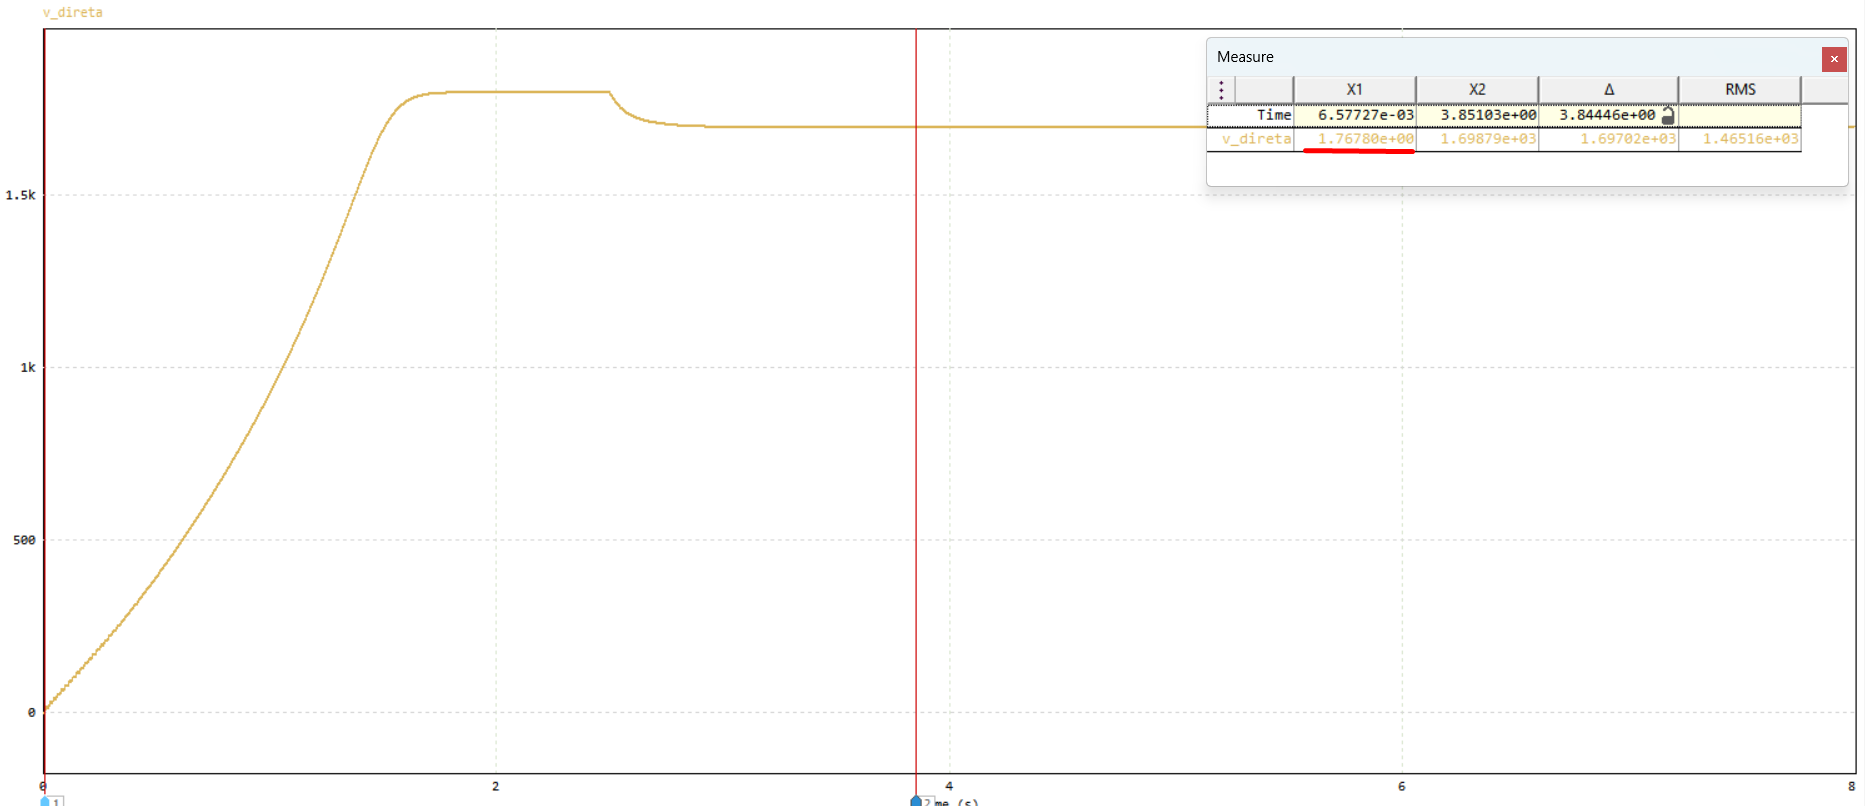
\includegraphics[width=1\linewidth]{images/velocidade_partida_direta.png}
    \caption{Velocidade Assíncrona na Partida Direta}
    \label{fig:vel_assinc_direta}
\end{figure}

\begin{figure}[h]
    \centering
    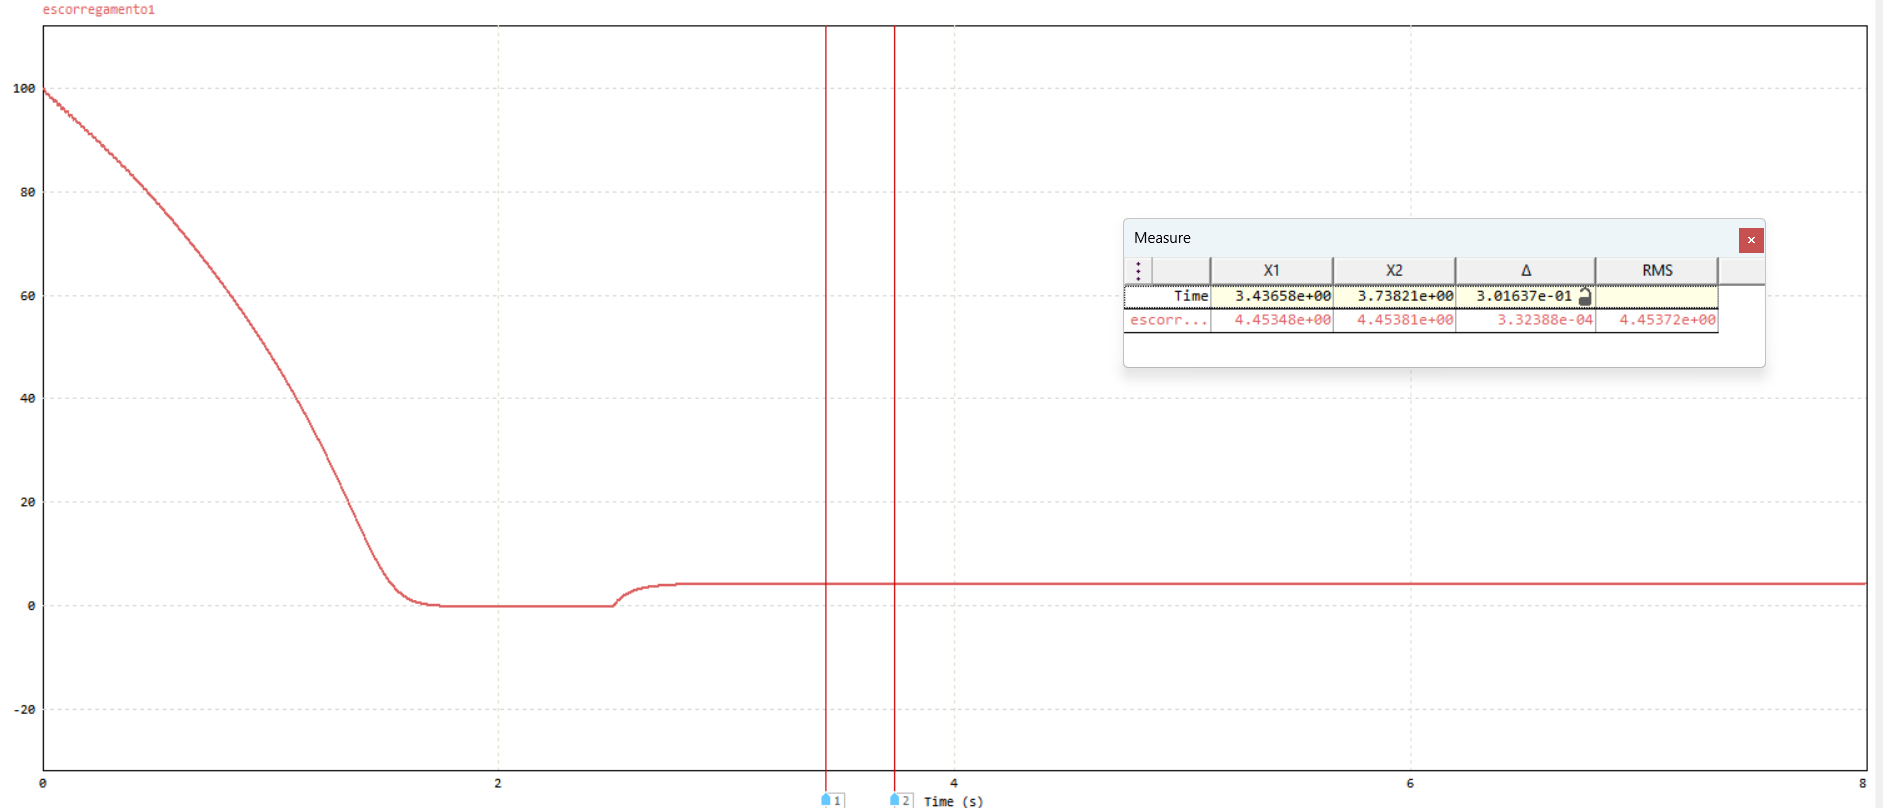
\includegraphics[width=1\linewidth]{images/escorregamento_direta.png}
    \caption{Escorregamento na Partida Direta}
    \label{fig:escorrega_direta}
\end{figure}


\section{Partida com inversor de frequência}

\subsection{Modulação por largura de pulsos senoidal}

O sinal SPWM (Modulação por Largura de Pulsos Senoidal) é essencial para o controle do inversor de frequência, determinando as características da saída alternada trifásica. O inversor utiliza chaves semicondutoras (IGBTs ou MOSFETs) dispostas em uma ponte trifásica para converter corrente contínua (DC) em corrente alternada (AC). A geração da saída AC é baseada no SPWM, que compara um sinal de referência senoidal ( $v_{\text {ref }}$ ) com uma onda portadora triangular ( $v_{\text {tri }}$ ) de alta frequência.

Quando $v_{\text {ref }}>v_{\text {tri, }}$ a chave correspondente é ativada, gerando alta ou baixa tensão no terminal do inversor, dependendo da polaridade. Esse processo é aplicado para cada fase, utilizando sinais de referência defasados em $120^{\circ}$, resultando em três fases moduladas na saída. A carga conectada, como um motor de indução, atua como um filtro passa-baixa, suavizando os harmônicos de alta frequência gerados pela modulação.

A tensão de saída do inversor em cada fase é dada por:

$$
V_f(t)=A \sin (\omega t), \quad A=\frac{m_a \cdot V_{C C}}{2}
$$

onde $m_a$ é o índice de modulação, que representa a relação entre a amplitude do sinal de referência senoidal e a amplitude da onda portadora triangular. O fator $m_a$ é limitado entre 0 e 1 para evitar distorções por saturação.
Com o índice de modulação $m_a$ fixado, o projeto do inversor foca no ajuste de $V_{C C}$ para atender às especificações de tensão de linha e frequência de operação, permitindo controle da velocidade angular do motor $(\omega(t))$ com apenas um grau de liberdade.

O circuito apresentado para acionamento de motores de indução é composto por dois módulos principais: o \textbf{módulo de geração do sinal de controle} e o \textbf{módulo inversor de frequência}.

O módulo de controle, ilustrado na Figura \ref{circuito sinal controle}, é responsável pela criação dos sinais PWM (Pulse Width Modulation) necessários para o acionamento do inversor de frequência. Ele utiliza a técnica de \textbf{modulação SPWM} (Modulação por Largura de Pulso Senoidal), conforme mostrado na Figura \ref{fig:spwm}. Este método consiste em comparar sinais senoidais trifásicos de referência, que definem a frequência e a amplitude de saída, com uma onda triangular de alta frequência, que determina o comportamento de chaveamento do inversor.

\begin{itemize}
    \item \textbf{Sinal senoidal de referência}: Gera tensões trifásicas defasadas em $120^\circ$ entre si. A frequência desses sinais determina a velocidade do motor e é ajustável para aplicações específicas.
    \item \textbf{Sinal triangular}: Gera uma onda portadora de alta frequência. A comparação com o sinal senoidal resulta nos pulsos PWM.
    \item \textbf{Resultado do SPWM}: Gera pulsos de controle trifásicos que modulam as chaves do inversor.
\end{itemize}

O inversor de frequência, representado na Figura \ref{fig:inversor_de_frequencia_conectado_motor}, é alimentado por uma fonte de corrente contínua e converte essa energia em uma saída alternada trifásica. Este módulo contém:

\begin{itemize}
    \item \textbf{Ponte H trifásica}: Estrutura composta por seis chaves semicondutoras (como IGBTs ou MOSFETs) que permitem a geração de tensões alternadas moduladas em amplitude e frequência.
    \item \textbf{Conversão CC-CA}: A modulação PWM gerada pelo módulo de controle é utilizada para chavear as chaves do inversor, transformando a tensão contínua do barramento em tensões alternadas trifásicas.
    \item \textbf{Filtragem natural}: A carga indutiva do motor suaviza as formas de onda PWM, resultando em tensões e correntes senoidais.
\end{itemize}
   
Os sinais PWM criados pelo módulo de controle entram no módulo inversor, que gera as tensões trifásicas moduladas para acionar o motor. A modulação SPWM permite controlar tanto a amplitude quanto a frequência das tensões fornecidas ao motor.

\begin{figure}[H]
    \centering
        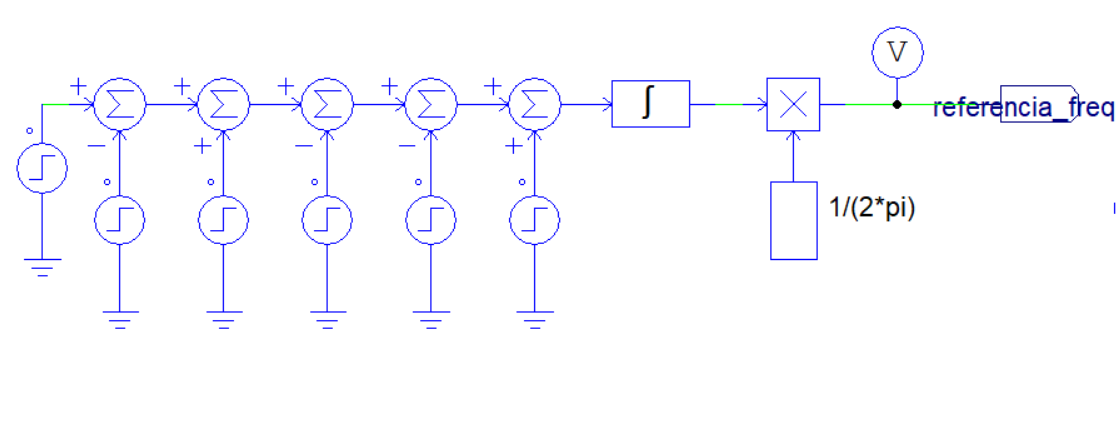
\includegraphics[width=1\linewidth]{images/circuito_referencia.png}
    \caption{Gerador do sinal de controle}
    \label{circuito sinal controle}
\end{figure}
  
\begin{figure}[H]
    \centering
    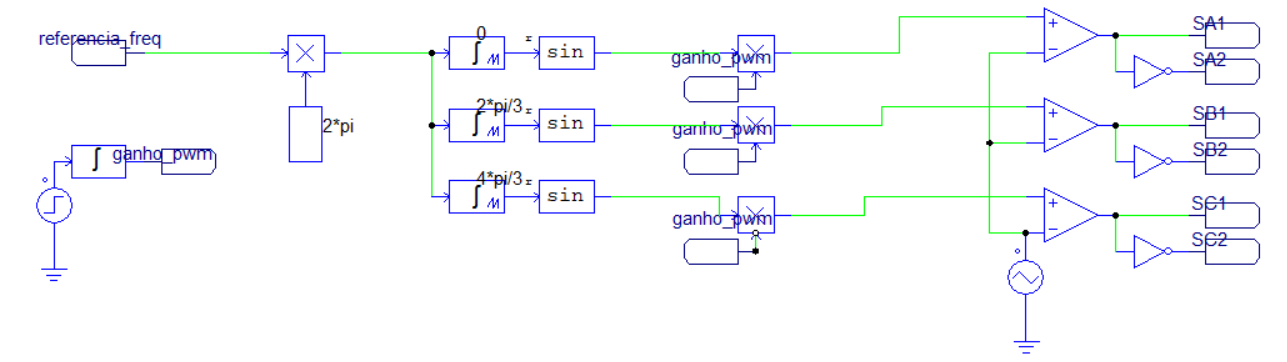
\includegraphics[width=1\linewidth]{images/spwm_2.png}
    \caption{Modulação SPWM (Sinusoidal Pulse Width Modulation) trifásica}
    \label{fig:spwm}
\end{figure}
  
\begin{figure}[H]
    \centering
    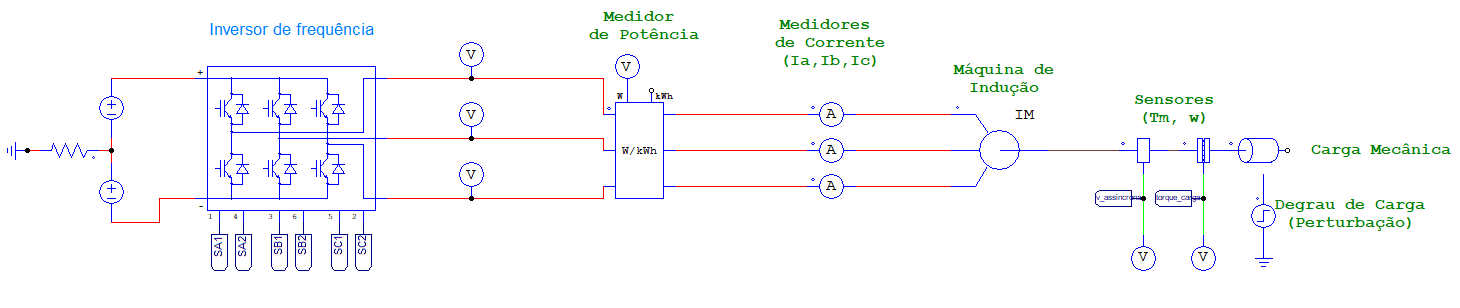
\includegraphics[width=1\linewidth]{images/inversor_de_frequencia_conectado_motor.png}
    \caption{Inversor de frequência conectado ao motor}
    \label{fig:inversor_de_frequencia_conectado_motor}
\end{figure}

\subsection{Parâmetros do projeto}

Os parâmetros do projeto foram definidos de acordo com os seguintes objetivos:

\begin{itemize}
    \item \textbf{Partida suave em rampa via inversor de frequência}: O pico de corrente deve ser limitado a no máximo 25\% do pico da corrente nominal C.A.
    \item \textbf{Potência nominal}: O motor deve alcançar uma potência de 12 kW após o acionamento em rampa (60 Hz, 220 Vrms - tensão de linha).
    \item \textbf{Cenário de variação da velocidade}: Inclui a variação da velocidade síncrona em malha aberta entre $-20 \%$ e $+20 \%$ da frequência nominal.
    \item \textbf{Velocidade síncrona}: Calculada com a fórmula:
    \[
    \omega_s = \frac{120 \cdot f}{N}
    \]
    onde $f$ é a frequência da rede e $N$ é o número de polos da máquina. Para 60 Hz e 4 polos, a velocidade síncrona é $\omega_s = 1800 \, \mathrm{RPM}$.
    \item \textbf{Escorregamento ($S$)}: Projetado para estar entre $2 \%$ e $6 \%$, conforme avaliado a partir do gráfico de velocidade mecânica em relação à síncrona:
    \[
    S = \frac{\omega_s - \omega_m}{\omega_s} \cdot 100 \%
    \]
    onde $\omega_m$ é a velocidade mecânica do motor.
\end{itemize}

O projeto implementado consiste em uma ponte 3 H conectada a um circuito de controle digital por PWM. O PWM foi configurado utilizando um comparador entre uma onda triangular, variando entre -1 e 1, e um sinal senoidal de referência, com amplitude ajustada para 0,9 e defasagem trifásica de $120^{\circ}$. A onda triangular foi definida com uma frequência de 3 kHz , garantindo que suas componentes harmônicas não interferissem na dinâmica da máquina, visto que o motor, do ponto de vista elétrico, atua como um filtro passa-baixa.

Para representar corretamente a onda triangular de 3 kHz no domínio do tempo, foi necessário escolher um passo de simulação baseado na frequência de Nyquist. A frequência de Nyquist é \(f_s = 2 f_\text{tri}\), onde \(f_\text{tri} = 3\,\mathrm{kHz}\), resultando em \(f_s = 6\,\mathrm{kHz}\). Para assegurar alta precisão na interação entre o sinal senoidal de referência e a onda triangular, foi utilizada uma frequência de amostragem 30 vezes maior que a frequência de Nyquist, \(f_s = 180\,\mathrm{kHz}\), correspondendo a um passo de simulação \(T_s = \frac{1}{f_s} \approx 5.56\,\mu s\).


Para atender à especificação de \( V_{LL, \text{rms}} = 220 \, \mathrm{V} \), foram utilizadas duas fontes simétricas de \( V_{CC} = 200 \, \mathrm{V} \) cada, totalizando \( V_{CC} = 400 \, \mathrm{V} \). O cálculo foi fundamentado nas relações do PWM trifásico:

A tensão de fase RMS (\( V_{\text{fase}, \text{rms}} \)) gerada pelo inversor em modulação por largura de pulso (PWM) é dada por:

\[
V_{\text{fase}, \text{rms}} = \frac{m_a \cdot V_{CC}}{2\sqrt{2}}
\]

\[
V_{LL, \text{rms}} = \sqrt{3} \cdot V_{\text{fase}, \text{rms}} \implies V_{LL, \text{rms}} = \sqrt{3} \cdot \frac{m_a \cdot V_{CC}}{2\sqrt{2}}
\]

Dado que \( V_{LL, \text{rms}} = 220 \, \mathrm{V} \) e o índice de modulação \( m_a = 0.9 \), a tensão total do barramento CC é calculada como:

\[
V_{CC} = \frac{2\sqrt{2} \cdot V_{LL, \text{rms}}}{\sqrt{3} \cdot m_a} = \frac{2\sqrt{2} \cdot 220}{\sqrt{3} \cdot 0.9} \approx 400 \, \mathrm{V}
\]

Portanto, cada fonte simétrica deve fornecer \( V_{CC} = 200 \, \mathrm{V} \). Essa configuração garante que o barramento CC seja suficiente para o correto acionamento do motor trifásico, permitindo que o inversor gere tensões senoidais equilibradas nas três fases. Além disso, a simetria das fontes reduz distorções na saída do inversor e mantém um neutro virtual estável, essencial para o equilíbrio entre as tensões positivas e negativas do barramento CC.

\subsection{Sinais de referência}
O sinal de controle $referencia\_freq$ foi projetado para levar o motor à proximidade da velocidade síncrona, que ocorre quando a frequência da tensão que alimenta o motor é da rede, ou seja, 60 Hz. Para facilitar a análise gráfica, o sinal foi inicialmente representado em Hz, dividindo sua escala em rad/s por \(2\pi\), e, para alimentar o circuito PWM, foi reconvertido para rad/s multiplicando novamente por \(2\pi\). A referência de frequência foi levada a 60 Hz em 3,0 segundos sem ultrapassar as restrições de corrente máxima. Durante a partida, são controladas tanto a frequência com o sinal $referencia\_freq$ quanto o ganho da senoide de referência do SPWM com o $ganho\_pwm$. Após o transiente da partida, o $ganho\_pwm$ é mantido constante como 0.9. Em 5 segundos, é aplicada a carga (perturbação). Em 7 segundos o sinal de referência começa a aumentar até passar a ser maior 20\% em relação ao nominal e em 9 segundos ele é reduzido em 20\%, esse sinal é ilustrado na Figura \ref{fig:sinal_ref_freq}.

\begin{figure}[H]
    \centering
    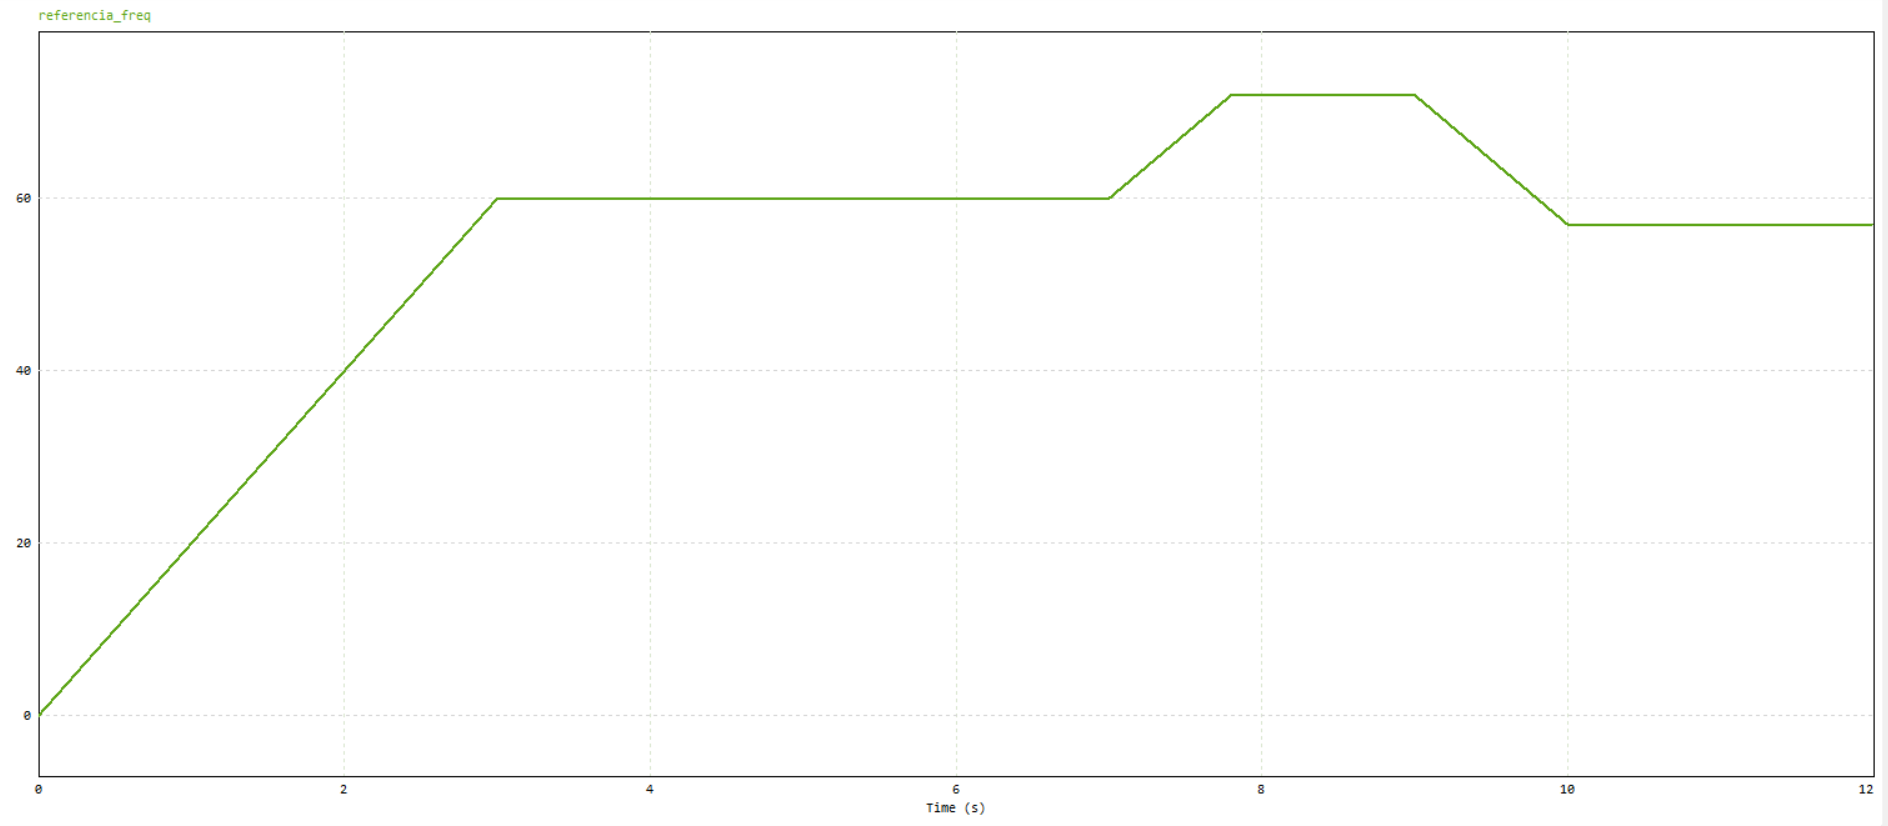
\includegraphics[width=1\linewidth]{correcao_images/corre_ref.png}
    \caption{Sinal referência de frequência em Hz. O ganho do PWM (ma) aumentou de 0 a 0.9 na rampa de 0 a 3 segundos para garantir a partida suave.}
    \label{fig:sinal_ref_freq}
\end{figure}

\subsection{Cálculo do torque}

Para alcançar a potência elétrica nominal (de regime permanente no intervalo entre 5.0s e 7.0s com aplicação da carga após a partida) desejada de \(12\,\mathrm{kW}\) com uma eficiência de \(90\%\) (\(\eta = 0.9\)), a potência mecânica (\(P_{\text{mec}}\)) foi calculada usando a relação:

\[
P_{\text{mec}} = \eta \cdot P_{\text{el}}.
\]

Substituindo \(P_{\text{el}} = 12\,\mathrm{kW}\) e \(\eta = 0.9\), obtemos:

\[
P_{\text{mec}} = 0.9 \cdot 12 = 10.8\,\mathrm{kW}.
\]

Com \(P_{\text{mec}}\) definido, o torque mecânico (\(T_m\)) foi calculado com base na velocidade angular do rotor (\(\omega_r\)). A velocidade do rotor (\(N_r\)) foi obtida pela fórmula:

\[
N_r = N_s \cdot (1 - S),
\]

onde \(N_s = 1800\,\mathrm{rpm}\) é a velocidade síncrona e \(S = 4\%\) é o escorregamento, resultando em:

\[
N_r = 1800 \cdot (1 - 0.04) = 1728\,\mathrm{rpm}.
\]

A velocidade angular do rotor foi calculada como:

\[
\omega_r = \frac{2\pi N_r}{60} \approx \frac{2\pi \cdot 1728}{60} \approx 180.96\,\mathrm{rad/s}.
\]

O torque mecânico necessário foi então obtido pela relação:

\[
T_m = \frac{P_{\text{mec}}}{\omega_r},
\]

resultando em:

\[
T_m \approx \frac{10.8 \cdot 10^3}{180.96} \approx 59.69\,\mathrm{Nm}.
\]

\subsection{Resultados}

Por meio da construção do circuito do inversor de frequência, da definição dos parâmetros do PWM e da geração dos sinais de referência necessários para alcançar as atuações desejadas, foi possível obter gráficos representativos que demonstram o desempenho do acionamento utilizando o inversor de frequência em comparação à partida direta, os resultados são apresentados nas subseções a seguir.

\subsubsection{Tensões de saída do inversor Va, Vb e Vc}

\begin{figure}[H]
    \centering
    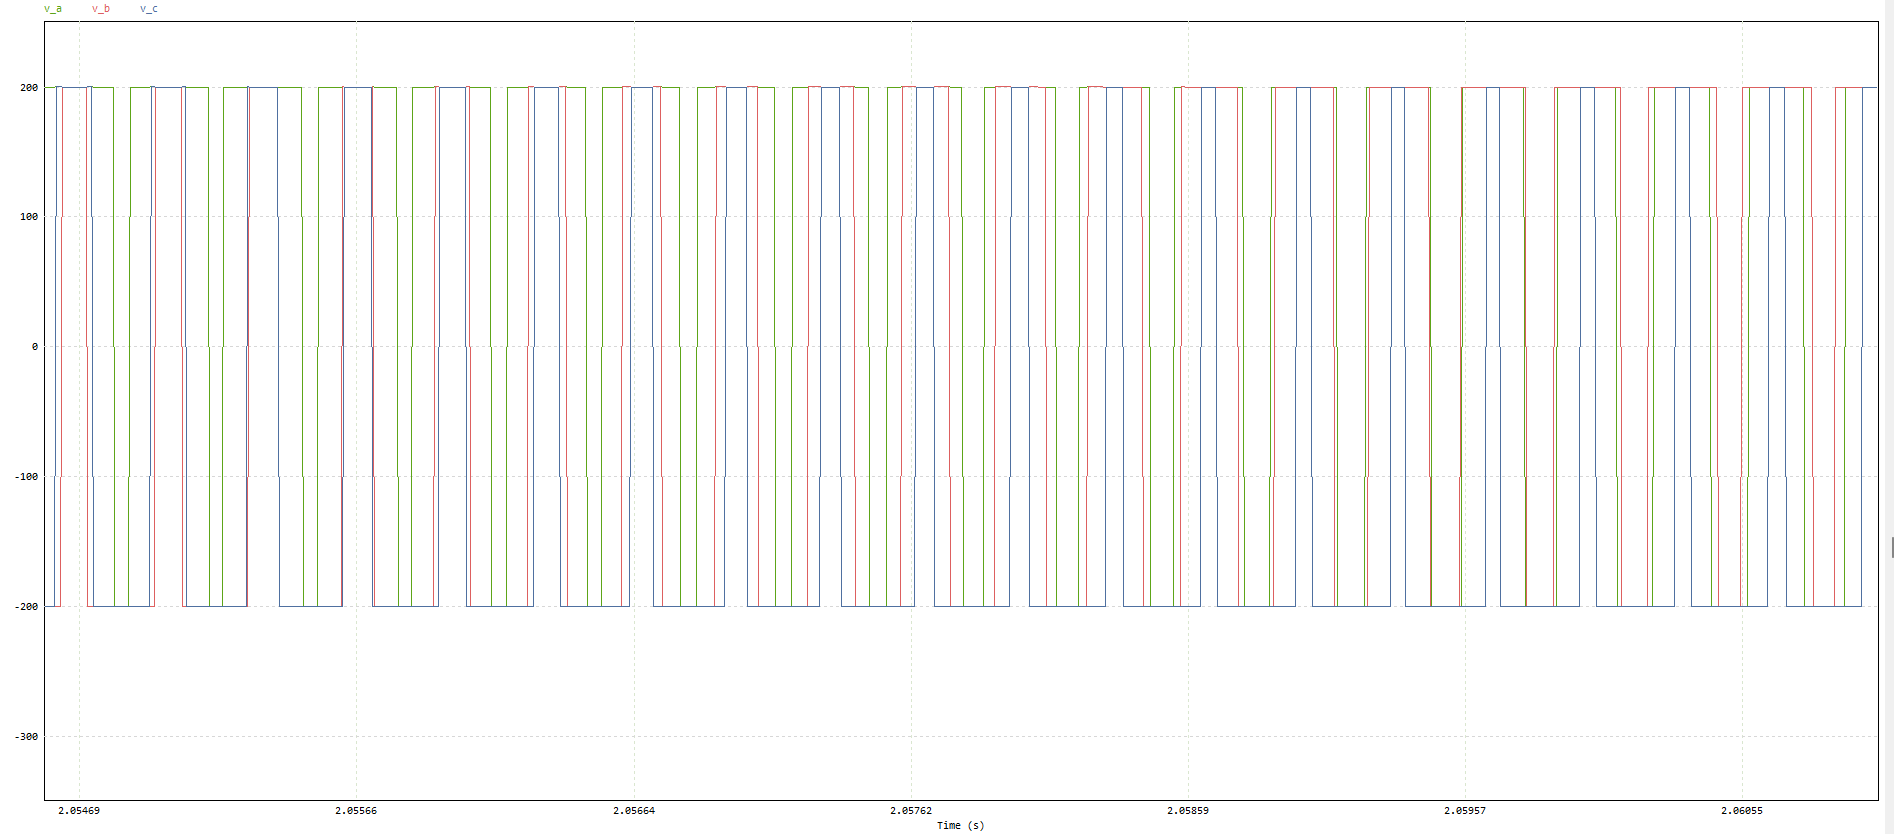
\includegraphics[width=1\linewidth]{correcao_images/tensoes_inversor.png}
    \caption{Tensões Inversor [V]}
    \label{fig:tensoes-inversor}
\end{figure}

\begin{figure}[H]
    \centering
    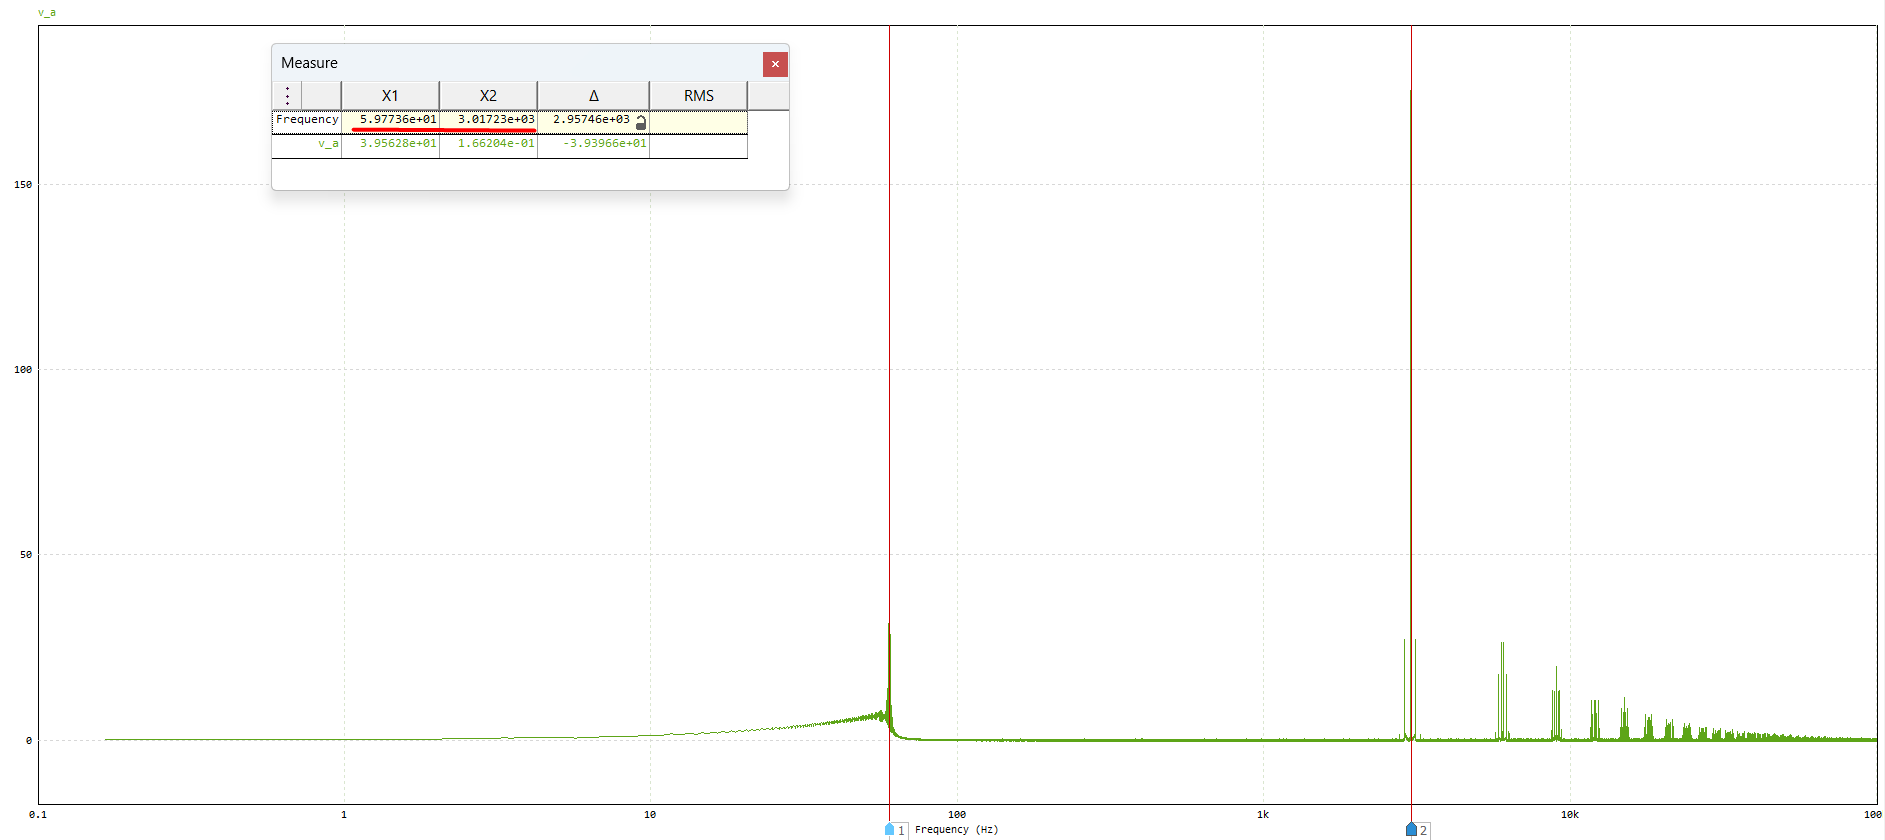
\includegraphics[width=1\linewidth]{fft_2.png}
    \caption{FFT do sinal de tensão na saída do inversor. É possível observar picos nas frequências de 60Hz e 3KHz}
    \label{fig:enter-label}
\end{figure}

A Transformada de Fourier (FFT) do sinal de saída do inversor de frequência evidencia não apenas o pico na frequência fundamental de 60 Hz, mas também um pico em 3 kHz, correspondente à frequência da portadora triangular utilizada na modulação. Isso ocorre porque a saída não é uma onda senoidal pura, mas sim um trem de pulsos resultante da comparação entre a senóide de referência e a onda triangular de alta frequência. Como consequência, a FFT mostra não só o componente fundamental, mas também a presença de harmônicas e bandas laterais em torno de 3 kHz e seus múltiplos, refletindo a natureza pulsada e modulada do sinal gerado pelo chaveamento.

\subsubsection{Correntes Ia, Ib e Ic}

No projeto do inversor de frequência, a corrente de pico durante o regime transiente foi de 59 A, representando uma redução de aproximadamente $75 \%$ em relação à corrente máxima de 236A observada na partida direta. Além disso, a corrente de pico foi cerca de $22 \%$ maior que a corrente nominal  (de regime permanente no intervalo entre 5.0s e 7.0s com aplicação da carga após a partida) de 48 A, atendendo ao critério de limitar o pico de corrente a $25 \%$ da corrente nominal.A Figura \ref{fig:corrente-maxim} ilustra a redução dos valores de corrente durante o transiente do acionamento com inversor em relação ao direto, e a corrente de pico obtida.


\begin{figure}[H]
    \centering
    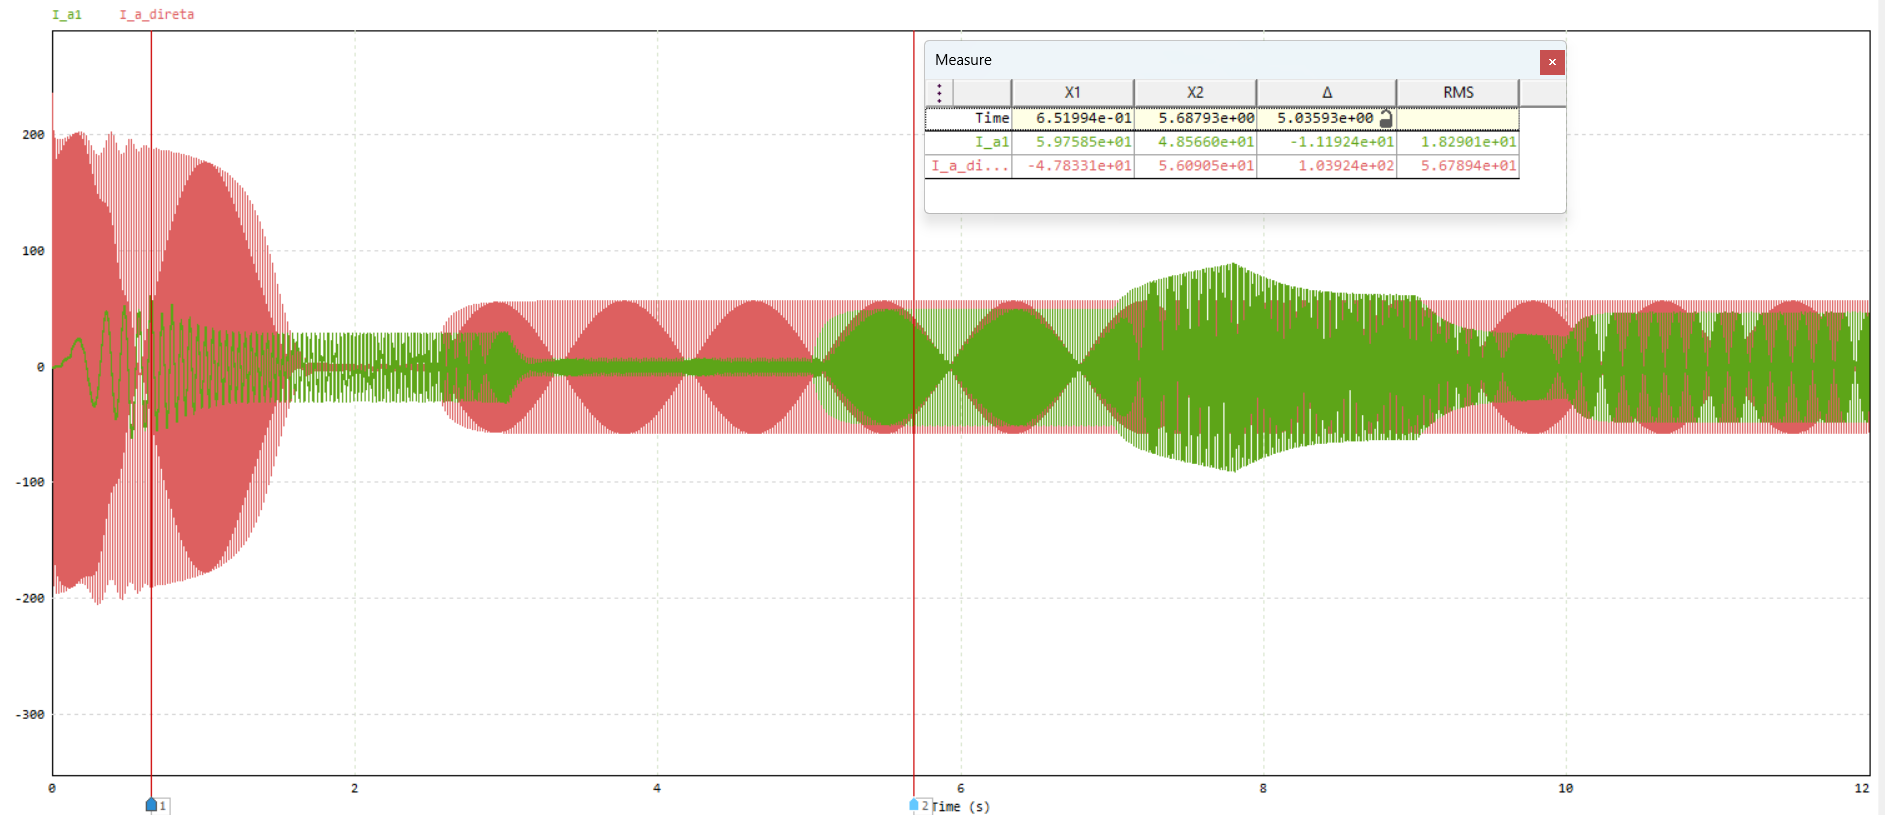
\includegraphics[width=1\linewidth]{correcao_images/corre_ia_max.png}
    \caption{Correntes Ia [A] com e sem inversor.}
    \label{fig:corrente-maxim}
\end{figure}

Já a figura \ref{fig:correntes com inversor} ilustra as três correntes CA com o uso do inversor de frequência nas diferentes condições:

\begin{itemize}
    \item Partida (regime transiente);
    \item Regime permanente;
    \item Aplicação de carga;
    \item Variação da frequência em $\pm$ 20\%
\end{itemize}

\begin{figure}[H]
    \centering
    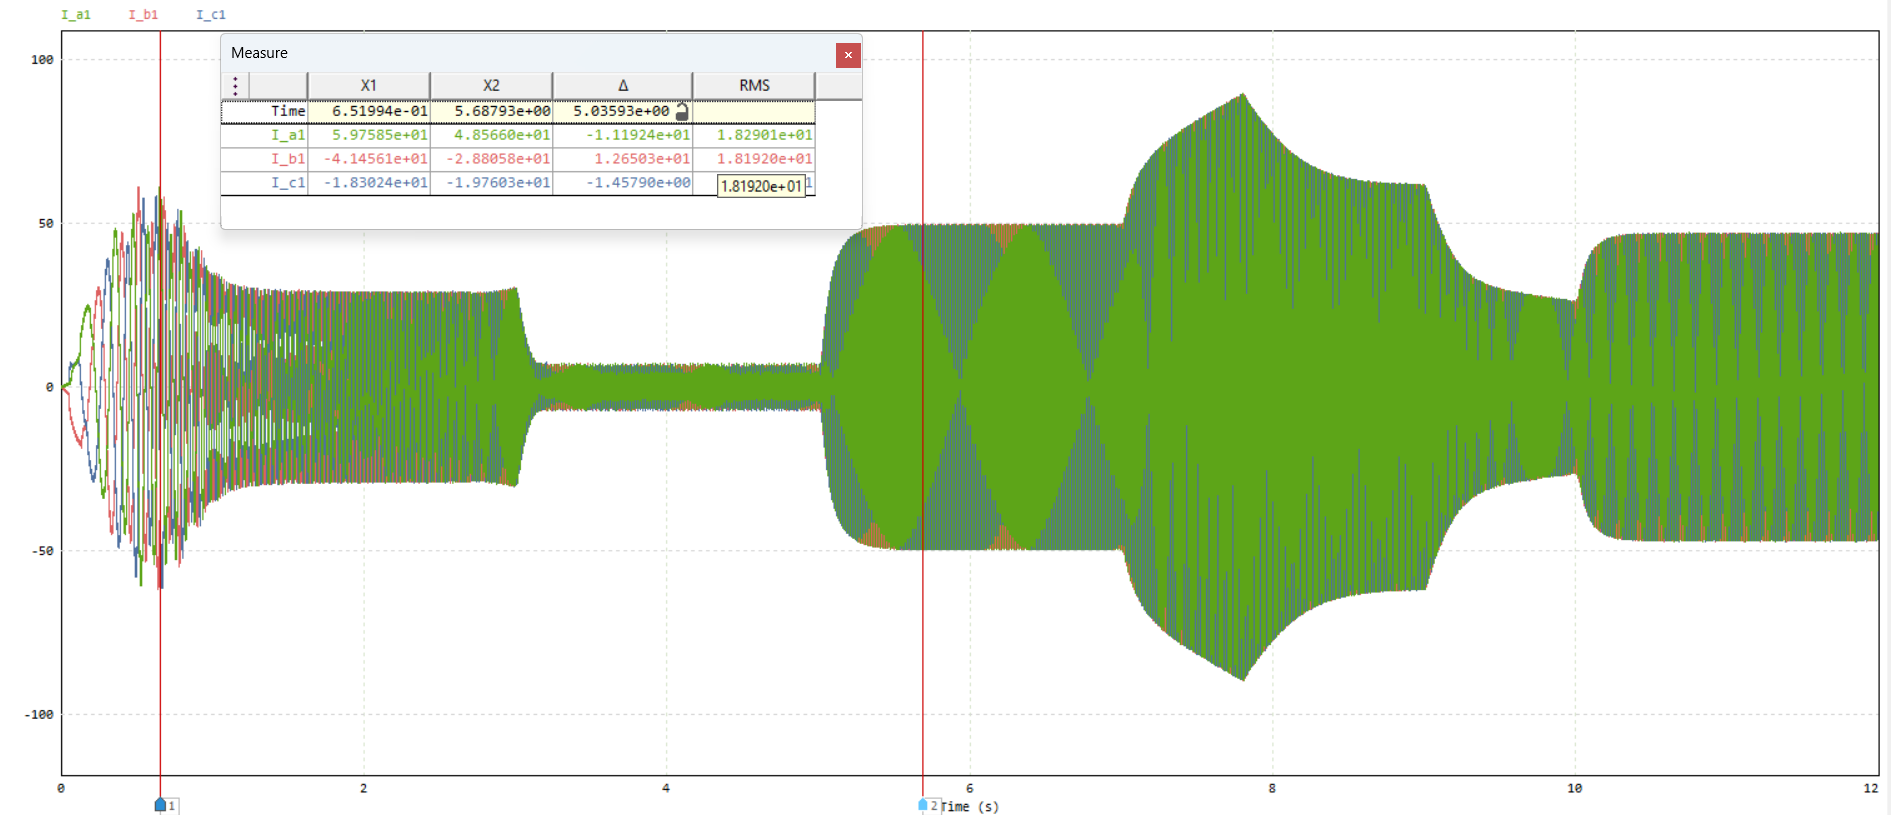
\includegraphics[width=1\linewidth]{correcao_images/todas_is.png}
    \caption{Correntes Ia, Ib e Ic [A] durante o acionamento por inversor de frequência.}
    \label{fig:correntes com inversor}
\end{figure}

Assim como no acionamento por partida direta, após o regime transiente (no qual o motor, que parte a vazio, alcança a velocidade nominal de 1800 RPM) as correntes trifásicas tendem a se aproximar de zero devido à ausência de carga. 

No instante de 5 segundos, é aplicada a carga de 59 N·m, resultando no aumento das correntes até que um novo regime permanente seja alcançado, com pico de corrente registrado em aproximadamente 48,56 A.

Posteriormente, no instante de 7 segundos, o sinal de referência de frequência aumenta em 20$\%$ em relação ao valor nominal, atingindo uma frequência de 72 Hz. Esse aumento explica o crescimento temporário das correntes até que a nova velocidade seja alcançada, momento em que as correntes voltam a diminuir, estabilizando-se novamente.

No entanto, no instante de 9 segundos, ocorre a redução do sinal de referência de frequência em 20$\%$ do valor anterior, atingindo o valor de 57,6 Hz, resultando em uma redução na velocidade do motor, mas também em um aumento das correntes após o regime transiente. Esse comportamento ocorre porque, com a redução da velocidade do motor, o escorregamento relativo ao campo magnético do estator aumenta, o que pode ser visto na figura \ref{escorrega}, levando a uma maior indução de corrente no rotor.

\subsubsection{Velocidades Síncrona e mecânica (assíncrona)}

Analisou-se ainda o comportamento das velocidades, ambas em rpm, conforme ilustrado na figura \ref{fig:velocidades}. 

\begin{figure}[H]
    \centering
    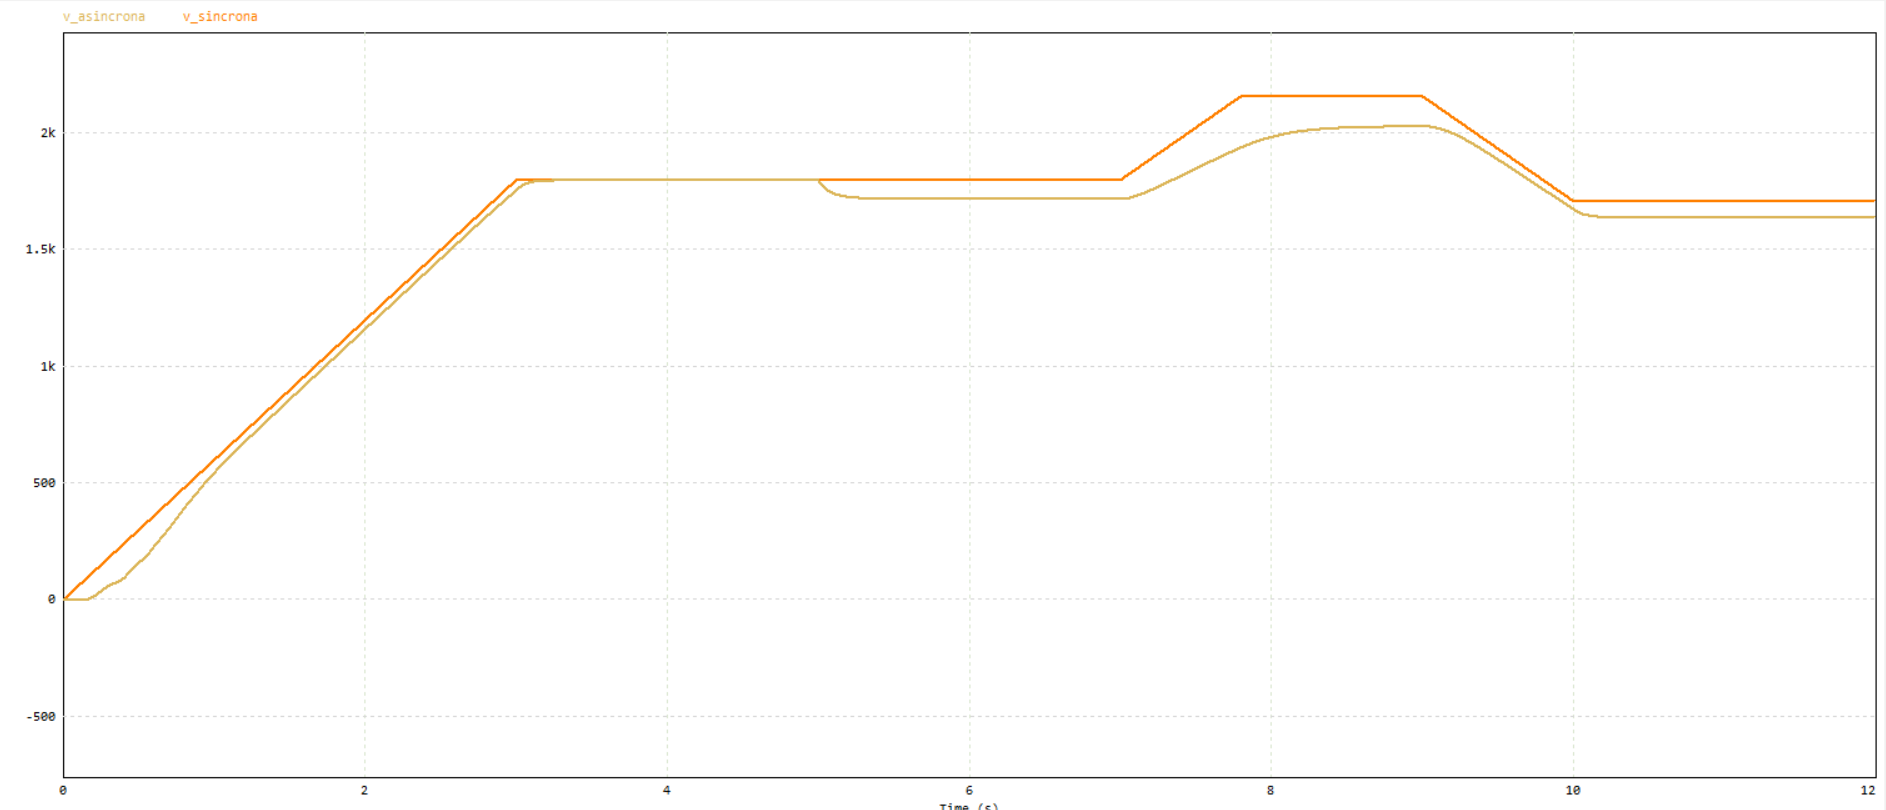
\includegraphics[width=1\linewidth]{correcao_images/corre_velocidades.png}
    \caption{Velocidade síncrona e mecânica [RPM].}
    \label{fig:velocidades}
\end{figure}

No gráfico, a velocidade síncrona segue o sinal de referência de frequência, o que significa dizer que os sinais são equivalentes, mas em unidades distintas. Por isso, a velocidade síncrona aumenta até 2160 RPM após o instante de 7s (aumento de 20$\%$ em relação ao valor nominal) e cai para 1728 RPM após o instante de 9s (redução de 20$\%$ em relação ao valor anterior).

É importante destacar que, em motores de indução, a velocidade síncrona é sempre maior que a velocidade do rotor (assíncrona). Essa diferença entre a velocidade do campo magnético rotativo gerado no estator e a velocidade do rotor é o que caracteriza o escorregamento, que está diretamente relacionado à geração de torque e ao desempenho do motor, influenciando sua eficiência.

\subsubsection{Escorregamento}

O projeto também chegou a um resultado de escorregamento dentro do intervalo esperado 2\% a 6\% conforme exibido na Figura \ref{escorrega}. O valor foi 4.4\% quando a referência de velocidade foi 60Hz, e 5.9\% quando o sinal de referência foi aumentado em 20\%. No gráfico, o escorregamento percentual aumenta em instantes onde há aumento da velocidade e consequentemente, geração de torque. 

\begin{figure}[H]
    \centering
    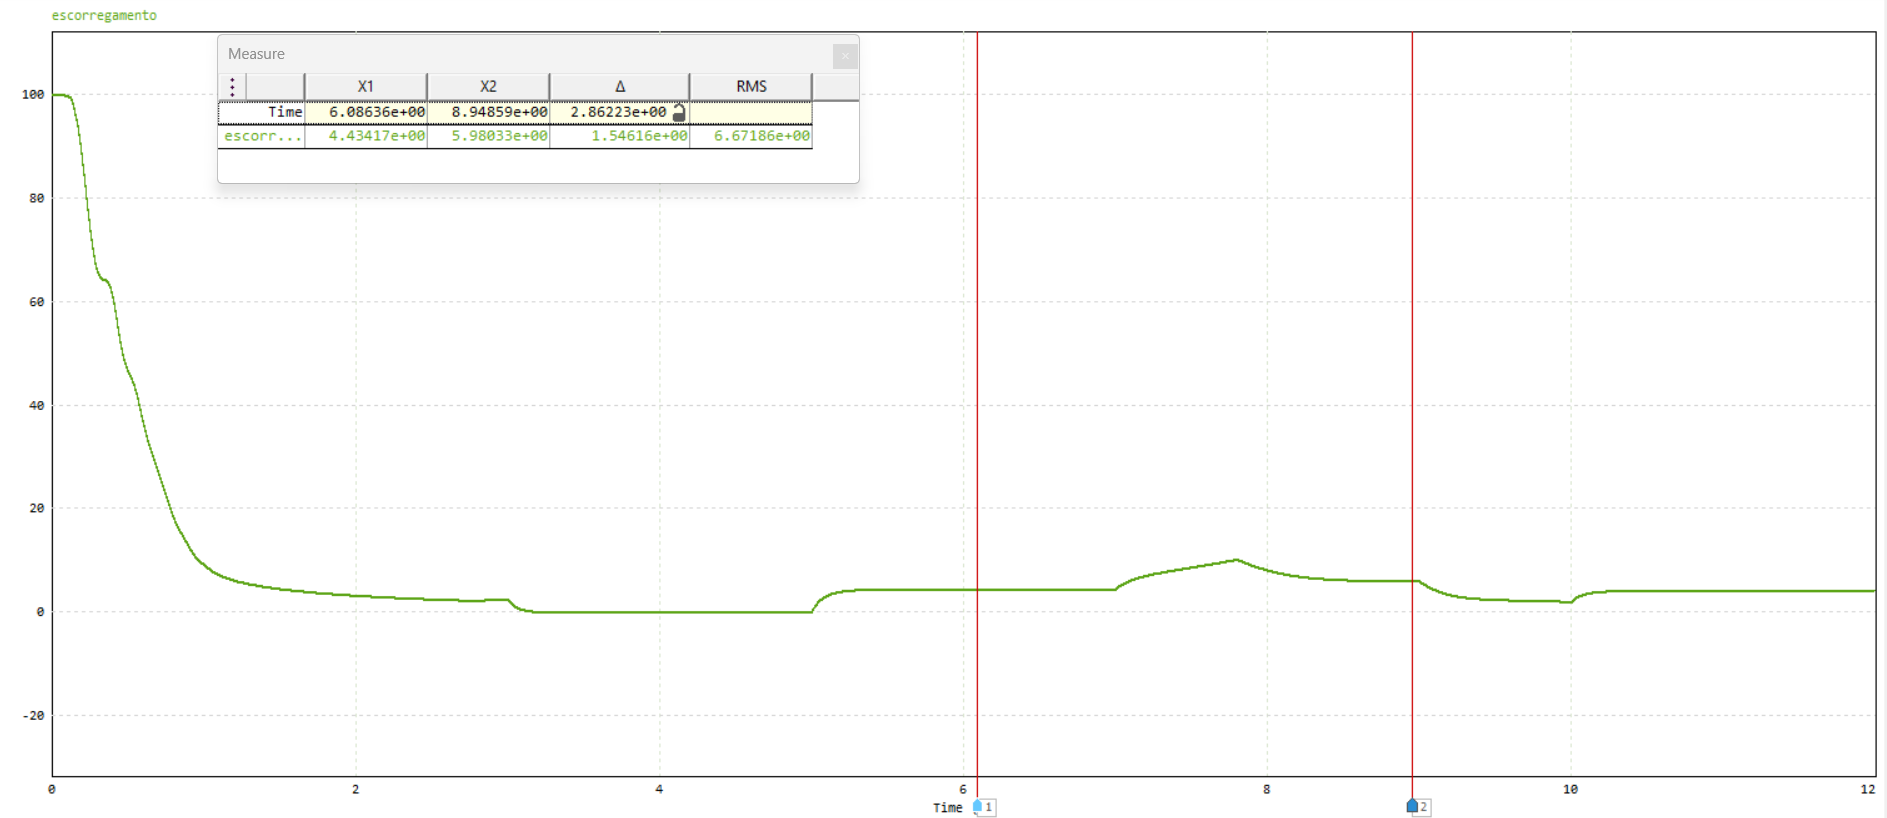
\includegraphics[width=1\linewidth]{correcao_images/corre_escorrega.png}
    \caption{Escorregamento percentual}
    \label{escorrega}
\end{figure}

\subsubsection{Potências Mecânica e Elétrica / Torque Elétrico e Mecânico }

Nas Figuras \ref{fig:torques} e \ref{fig:potencia} é possível observar que os houve um ajuste fino no torque de carga para que as potências batessem com os valores projetados.

\begin{figure}[H]
    \centering
    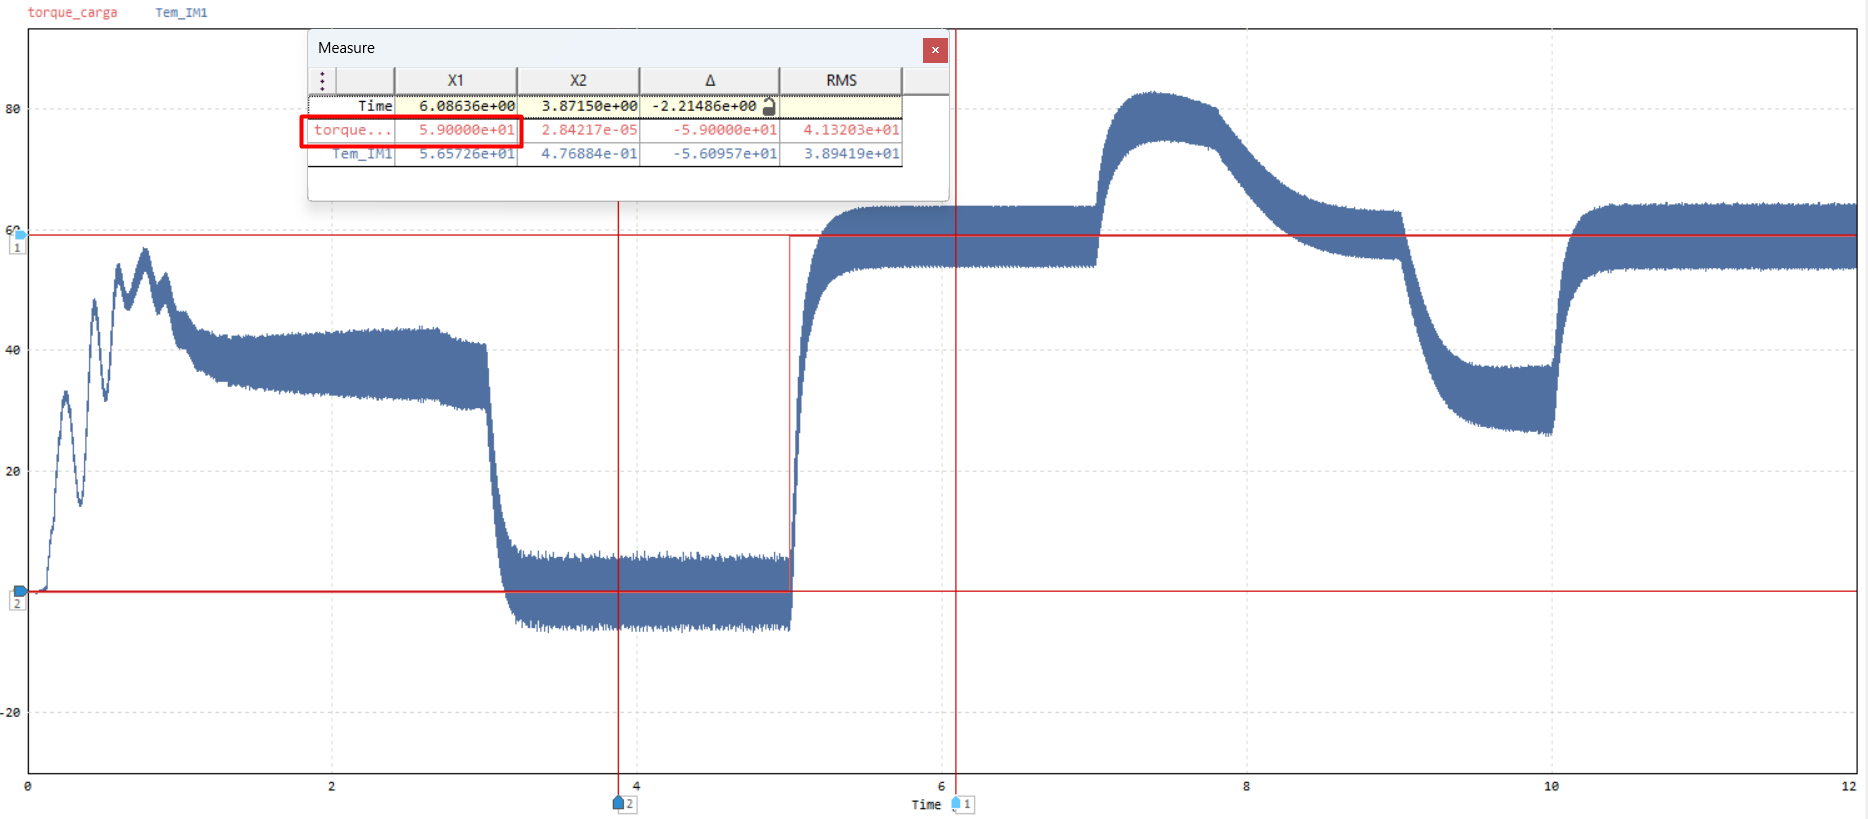
\includegraphics[width=1\linewidth]{correcao_images/corre_torque.png}
    \caption{Torque elétrico (azul) vs torque mecânico (vermelho) [N.M].}
    \label{fig:torques}
\end{figure}

Assim como representado pelo gráfico, tendo como momento inicial a inércia do motor, o torque aumenta no período de 0 a 3 segundos. Após esse período, uma vez que a velocidade se tornou constante e ainda não foi aplicada uma carga, o torque é reduzido pra zero. A partir do instante de 5 segundos é aplicada a carga e para levá-la a velocidade desejada o torque torna a subir. Com o aumento da velocidade em 20\% a partir dos 7 segundos o torque aumenta com o objetivo de levar a carga a essa nova velocidade, até esta se torne constante para então retornar ao valor de regime permanente. Da mesma forma, para uma redução da velocidade, o torque diminui até que a velocidade desejada seja observada, para então entrar novamente em regime permanente. 

\begin{figure}[H]
    \centering
    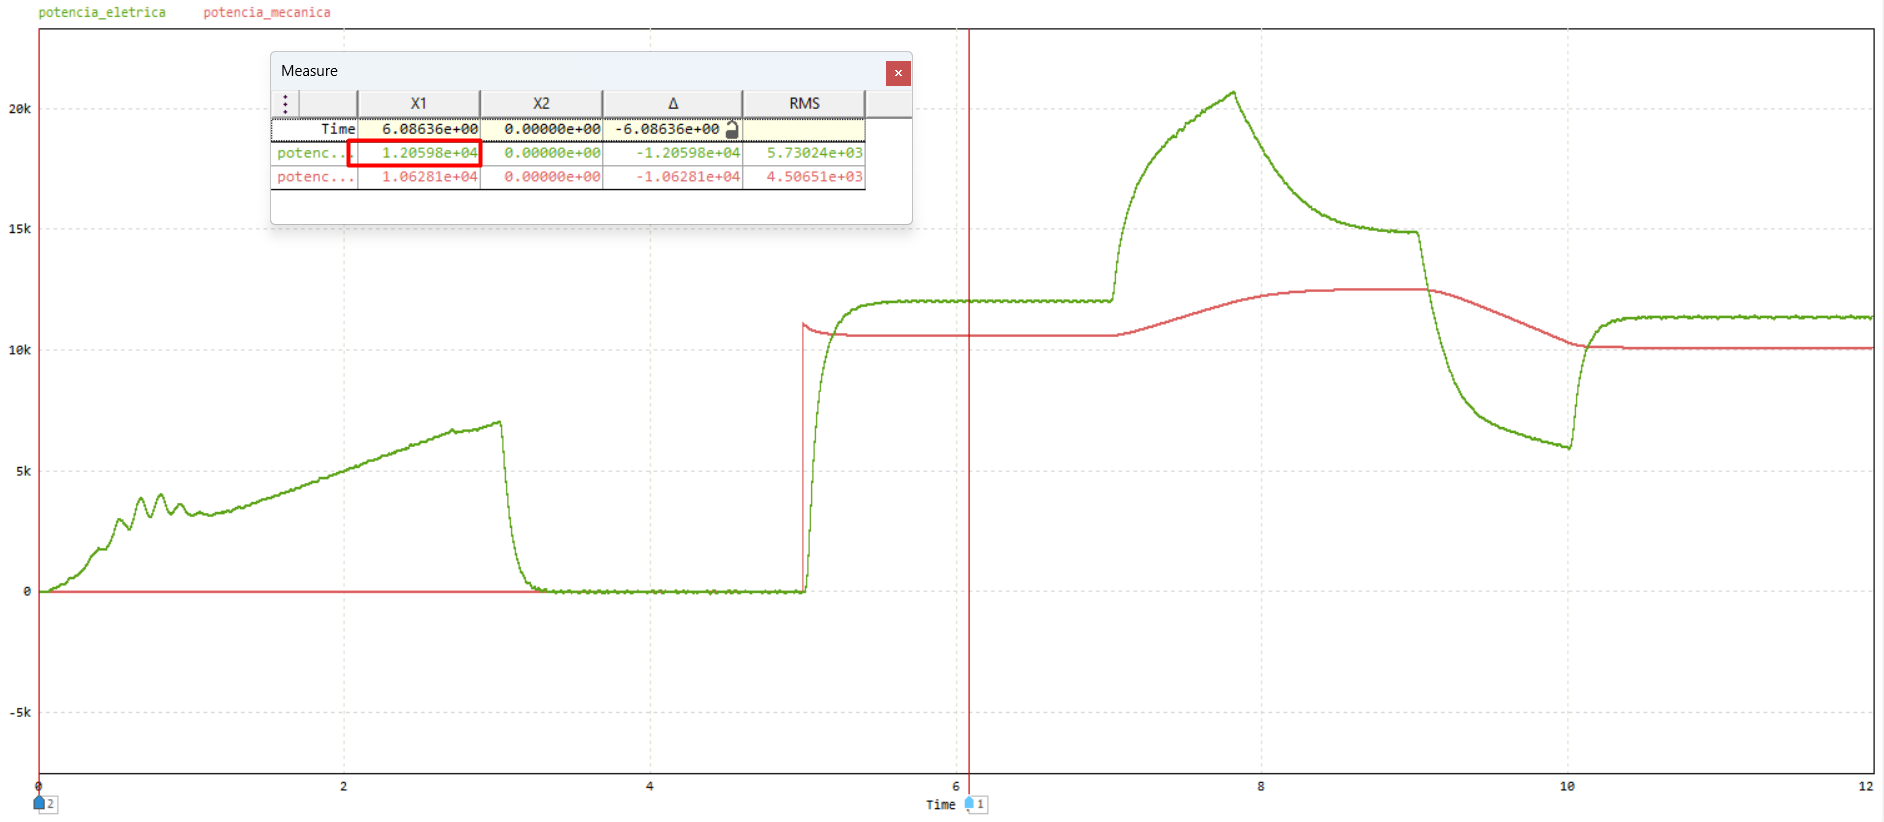
\includegraphics[width=1\linewidth]{correcao_pot.png}
    \caption{Potência elétrica X Potência mecânica [W]}
    \label{fig:potencia}
\end{figure}

\end{document}